\documentclass[11pt,a4paper]{report}

% Aberstwyth dissertation LaTeX Template
% Authors: Dr. Hannah Dee (hmd1@aber.ac.uk), Neil Taylor (nst@aber.ac.uk)
% This has been adapted from the Leeds Thesis template and the 
% Group Project template for Computer Science in Aberystywth University.
% 
% All comments and suggestions welcome.
%
% Template designed to be used with pdflatex: it may need alteration to
% run with a different LaTeX engine

% To build document on the unix command line, run four commands:
 
% pdflatex dissertation
% bibtex dissertation
% pdflatex dissertation
% pdflatex dissertation

% you will end up with dissertation.pdf 
\usepackage{mmp}
\usepackage{palatino}

% the following packages are used for citations - You only need to include one. 
%
% Use the cite package if you are using the numeric style (e.g. IEEEannot). 
% Use the natbib package if you are using the author-date style (e.g. authordate2annot). 
% Only use one of these and comment out the other one. 
\usepackage{cite}
%\usepackage{natbib}

% Use the following to selectively exclude chapters
%\includeonly{cover,abstract,acknowledge,declare,chapter1,chapter2}

\begin{document}

% all of the include directives below refer to tex files
% so 
\title{}

% Your name
\author{Theodoros Nikopoulos-Exintaris}

% Your email 
\authoremail{thn2@aber.ac.uk}

\degreeschemecode{GG47} %e.g. G400 
\degreeschemetitle{Computer Science} % e.g. Computer Science
\degreetype{BSc}

\modulecode{CS39440} % i.e. CS39440, CC39440, CS39620
\moduletitle{Major Project} % i.e. Major Project or Minor Project

\date{4th May 2016} % i.e. the date of this version of the report

\status{Draft} % Use draft until you create the release version. Then, change this to Release.
\version{1.0}

%The title and name of your supervisor.
\supervisor{Dr./Prof. Chuan Lu} 

%The email for your supervisor. 
\supervisoremail{cul@aber.ac.uk}

\maketitle



 includes cover.tex - to change the content,
% edit the tex file

\pagenumbering{roman}

% This is the front page

\title{}

% Your name
\author{Theodoros Nikopoulos-Exintaris}

% Your email 
\authoremail{thn2@aber.ac.uk}

\degreeschemecode{GG47} %e.g. G400 
\degreeschemetitle{Computer Science} % e.g. Computer Science
\degreetype{BSc}

\modulecode{CS39440} % i.e. CS39440, CC39440, CS39620
\moduletitle{Major Project} % i.e. Major Project or Minor Project

\date{4th May 2016} % i.e. the date of this version of the report

\status{Draft} % Use draft until you create the release version. Then, change this to Release.
\version{1.0}

%The title and name of your supervisor.
\supervisor{Dr./Prof. Chuan Lu} 

%The email for your supervisor. 
\supervisoremail{cul@aber.ac.uk}

\maketitle



                        

% Set up page numbering
\pagestyle{empty}

% declarations of originality 
\thispagestyle{empty}

%%%
%%% You must sign the declaration of originality. 
%%%
\begin{center}
    {\LARGE\bf Declaration of originality}
\end{center}

In signing below, I confirm that:

\begin{itemize}
\item{This submission is my own work, except where 
clearly indicated.}

\item{I understand that there are severe penalties for 
Unacceptable Academic Practice, which can lead to loss 
of marks or even the withholding of a degree.}
 
\item{I have read the regulations on Unacceptable Academic 
Practice from the University's Academic Quality and 
Records Office (AQRO) and the relevant sections of the 
current Student Handbook of the Department of 
Computer Science.}
 
\item{In submitting this work I understand and agree to 
abide by the University's regulations governing these issues.}
\end{itemize}

\vspace{2em}
Name ............................................................  \\

\vspace{1em}
Date ............................................................ \\

%%% 
%%% We would like to make a selection of final reports available to students that take 
%%% this module in future years. To enable us to do this, we require your consent. You 
%%% are not required that you do this, but if you do give your consent, then we will have 
%%% the option to select yours as one of a number of reports as examples for other 
%%% students. If you would like to give your consent, then please include the following 
%%% text and sign below. If you do not wish to give your consent, please remove this 
%%% from your report. 
%%%
\vspace{1em}
\begin{center}
    {\LARGE\bf Consent to share this work}
\end{center}

In signing below, I hereby agree to this dissertation being made available to other
students and academic staff of the Aberystwyth Computer Science Department.  

\vspace{2em}
Name ............................................................  \\

\vspace{1em}
Date ............................................................ \\


               

\thispagestyle{empty}

\begin{center}
    {\LARGE\bf Acknowledgements}
\end{center}

I'd like to thank Keiron O' Shea and Prof. Chuan Lu for volunteering to answer questions regarding neural networks and providing useful feedback and bibliography to get started on the topic.

The figure of a CNN architecture is taken from:
http://systemdesign.altera.com/can-you-see-using-convolutional-neural-networks/ % Acknowledgements
\thispagestyle{empty}

\begin{center}
    {\LARGE\bf Abstract}
\end{center}

Include an abstract for your project. This should be no more than 300 words.
                 % Abstract

\pagenumbering{roman}
\pagestyle{fancy}
\fancyhead{}
\fancyfoot[C]{\thepage}
\renewcommand{\headrulewidth}{0 pt}
\renewcommand{\chaptermark}[1]{\markboth{#1}{}}

\tableofcontents   
\newpage
\listoffigures
\newpage 
\listoftables
\newpage

% Set up page numbering
\pagenumbering{arabic}

\setchapterheaderfooter

% include the chapters
\chapter{Background \& Objectives}

\section{Introduction}
This project is an investigation into training Artificial Neural Networks for the purpose of image classification and labelling. We will explore alternative approaches in computer vision to solve this problem arriving to the what is considered the current state of the art in machine learning, comparing it to a number of different alternatives, both contemporary but also historical.

\subsection{Motivation}
Perhaps the first question we might wish to ask ourselves is "why we wish to embark on this project in the first place". Computer vision is a field of computer science in essence, involving extracting information and building models of the real world; this might involve sensors, cameras or perhaps even audio.

There are numerous applications and types of computer vision. The problem we are looking in particular is identifying images and labelling them, extracting metadata from the image itself. Naturally this has many applications. Self-driving cars, search engines, and any problem where we need a computer to be able to identify images.

Our interest is particularly related to image acquisition and labelling. Suppose a user has a large set of images and you are looking for a particular one. They know what it is but not its title. Or perhaps its title does not hold semantic meaning to them, but wish to search the semantics of the image itself.

\subsection{Machine Learning and Pattern Recognition}
To solve this problem, computer scientists set out to devise a set of 'rules' and algorithms that were good at solving these problems. Eventually, it became apparent that no single algorithm could solve the problem for all sets of cases as the 'rules' change between cases. The rules that define a cat are different the ones that define a dog and so on, so one would have to write rules for each edgecase. Where you needed to solve this kind of problem one would analyse the data they expect to receive and think of features they are interested in extracting. This approach is still used for some CV problems.

A solution that emerged for this was machine learning $\left(ML\right)$, that is sets of algorithms that could be used to derive the rules based on data. Most machine learning algorithms work by identifying patterns in the data, either via statistical analysis as in Bayesian Learning, or other means. Suppose you have a set of data describing cats and dogs. Cats are small, but there is both small and large types of dogs. Most cats have pointed ears while some dogs have floppy ones. A machine learning algorithm would process a set of examples of cats and dogs, then it would derive patterns that can be used to classify them.

\section{Background}
\subsection{SVMs and other Machine Learning Alternatives}
To use an SVM and most other ML methodologies, you begin by extracting the features you wish to learn from. If for example you are looking at a shape classifier, you would begin by considering what defines your classes. For this example, perhaps the number of edges might be a feature, perhaps the relative length of each straight edge, or maybe the number of detected straight edges.

These can be extracted from an image using computer vision techniques, or in principle, machine learning would be used in a table of features that have already been extracted. Extracting features can be quite challenging on its own and can take a lot of effort. Having extracted the features however,  it is easy to gain insight on the decisions a ML algorithm makes.

\subsection {Artificial Neural Networks}
Artificial Neural Networks$\left(ANN\right)$ are a type of machine learning inspired by the way some biological organisms process stimulus and learn. In essence an ANN is a very naive emulation of a "meat computer", with the biological processes being replaced with mathematical approximations of the actual process of biological neurons.

Being that these are only approximations, they have several components which help them function and emulate select processes of real neurons.

\subsubsection{Advantages and Disadvantages of ANNs}
ANNs have many advantages and disadvantages to conventional ML methods. 

Some of the most important ones include: 
\begin{itemize}
	\item They do not require a feature extraction step
	\item They can easily be applied in many different problems
\end{itemize}
It is possible to apply ANNs in to solve many problems, by just feeding in appropriate training data and get reasonably accurate results in some cases, matching the state of the art for that problem.

As for disadvantages:
\begin{itemize}
	\item They are difficult to train both in terms of requirements and speed
	\item It is comparatively difficult to gain insight on why a neural network has learned something
\end{itemize}
Recent advances in ANNs have greatly improved on both of these areas. GPU compute in particular, has made training quite large neural networks practical, on consumer computers. There is also very active research at the moment in improving insight and visualising neural network decisions. We aim to talk in more detail about all of these later in our report.

\subsubsection{Datasets}
With most methodologies having data to test against is important. With ML, data is what drives the whole process so to produce any sort of solution to this problem one needs to decide on the dataset to use. For classification problems a dataset might be a set of inputs and outputs, separated in a set to train on and a set to test performance against afterwards.

For our network we are looking at datasets with actual images with associated labels. There is several of that type of image dataset, we will discuss them in more detail in a later section of this report.

\section{Analysis}
To complete this project, we must solve a number of problems and answer a number of questions. As part of our analysis we identified some of them, while several others would emerge as we embarked on our project.

\subsection{Types of ML and ANN architectures in use}
To start we should look at what models have been successful in the past for this kind of problem. After all this area has several decades of research behind it which we would not be able to replicate from scratch.

Looking at older results also enables us to get a baseline for what our model might be capable of doing and provides goals to hit or exceed. For this report we will be looking at SVMs, Multi Layer Perceptrons $\left(MLP\right)$ and Convolutional Neural Networks $\left(CNN\right)$

\subsection{Variables to test and optimise}
We need to decide on the architecture of our neural network. For CNN choices appear to be relatively simple, with most networks opting for very similar architectures. However, there are still aspects that can be varied.

We will need to investigate different ways we can vary our model and attributes that we can change in order to limit the scope of the research area. This process involves, reading documentation for our solutions as well as research into the technology we are using to determine the highest value optimisations to make.

\subsection{Are CNNs ready for market?}
One other interesting question to answer, as a conclusion, is whether CNNs are ready to be deployed in commercial products and services. Is it possible to produce something robust enough for such uses?

\section{Research Method}
To tackle any large undertaking, whether it is by a team of a single developer and their tenacity, or involving a team of expert code acrobats working in unison, we as developers, require a set of routines and rituals; this project is no different.

Prompted by a discussion on our Agile Methodologies module, we begun thinking Agile as a solution to this problem. We concluded that Agile would be appropriate to the spirit of our project, however due to this being a solo endeavour, we opted not to adopt any mainstream Agile methodologies. What we did instead is: we took elements we liked from Extreme Programming and combined them with parts of Scrum to create a methodology more closely tailored to our project.

What we needed was a way to drive quick prototyping and creative experimentation in a controlled manner, such that we could plan experiments while maintaining a rudimentary level of quality; while the nature of this project does not necessarily require the end product to be production-ready, since there is no customer nor a production environment. However, poor software quality would only hinder the experimental progress.

In our 'creative experimentation' process, we incorporate the concept of a sprint, but since we expect to go through a small iteration daily, we restrict time to the equivalent of a weekly sprint. Because we lack customers and a product owner, we replace them with our supervisor reporting progress after each week's sprint. The discussion is used to drive the direction and goals of the next sprint.

\begin{wrapfigure}{r}{0.21\textwidth}
	\begin{center}
		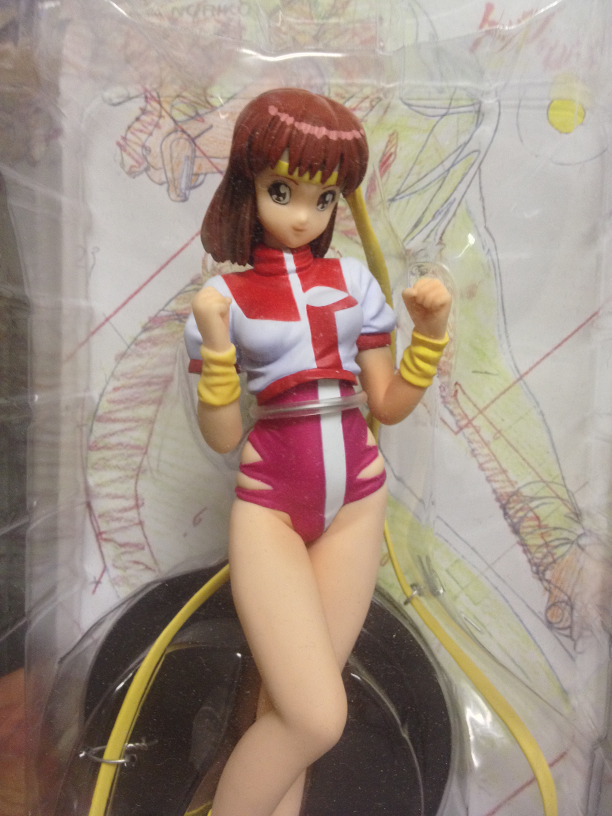
\includegraphics[width=0.19\textwidth]{hard_work_and_guts_programming}
	\end{center}
	\caption{A Pretty Soldier of Hard Work and Guts: Takaya Noriko.}
	\label{hwng}
\end{wrapfigure}

We are also using a form of continuous integration to deploy our changes, and GIT source control to track changes and experiments. We evaluate progress based on feedback from results and from milestones at the end of each 'sprint'. We considered Github issues as well but the were considered superfluous. Polyvinyl Carbonate Figure Debugging was implemented however. See fig. \ref{hwng}

The overall lifecycle looks like this:
\begin{itemize}
	\item First few cycles are exclusively dedicated to research and coming up with a set of requirements for the test infrastructure and programs that need to be developed to drive the project.
	\item After this we focus on designing and testing models with the aid of the basic software we designed in stage 1.
	\item New features will be added as needed to advance the project. Data loading, performance monitoring visualisation etc.
\end{itemize}


For experiments we begin to identify the variables and results we wish to test e.g. size of convolutional filters, then we identify the pre-requisites to run the tests. i.e. do we have the framework to run the experiment, and of course the desired data and whether we can extract them. For the third one we found that there was no need to add more output to run some experiments in our scope. Based on the results of an experiment we decide on what other experiments to run afterwards. Since experiments can take many hours to run, we need to plan a maximum of 2 experiments, a day with a expectation of perhaps doing less on some days or more on others.

Finally, we planned some basic overall schedule we use in 3 major milestones, research, implementation and writeup. Adjustments were to be made based on progress, initial planning was to use 2 weeks for research, 6 weeks for experiments and additional research as needed and 4 weeks for the report.

We have decided to name this methodology 'Hard Work and Guts Programming'. In the spirit of this, we are using this figurine of Takaya Noriko from the 1988 OVA 'Aim for the Top! Gunbuster' as poster child and rubber duck debugging surrogate $\left( fig. \ref{hwng} \right)$
%\addcontentsline{toc}{chapter}{Development Process}
\chapter{Experiment Methods}

This section should discuss the overall hypothesis being tested and justify the approach selected in the context of the research area.  Describe the experiment design that has been selected and how measurements and comparisons of results are to be made. 

You should concentrate on the more important aspects of the method. Present an overview before going into detail. As well as describing the methods adopted, discuss other approaches that were considered. You might also discuss areas that you had to revise after some investigation. 

You should also identify any support tools that you used. You should discuss your choice of implementation tools or simulation tools. For any code that you have written, you can talk about languages and related tools. For any simulation and analysis tools, identify the tools and how they are used on the project. 

If your project includes some engineering (hardware, software, firmware, or a mixture) to support the experiments, include details in your report about your design and implementation. You should discuss with your supervisor whether it is better to include a different top-level section to describe any engineering work.  
%\addcontentsline{toc}{chapter}{Development Process}
\chapter{Experiment Implementation}
\section{Summary}
To produce this research experiments must be run, and for this to happen experiments and the framework to carry them out need to be designed and implemented. This chapter will explain the key decisions and work carried out to produce our experimental results.

\section{Choice of Dataset}
For any machine learning task one of the first tasks that need to be undertaken once the nature of the task is determined is finding an appropriate dataset. The choice of dataset is important as it can dictate a number of our later decisions.

For image classification and labeling problems three of there are three common datasets that are used. We will briefly detail each one and choose which one to use.

There are of course other alternatives out there but these have been around for reasonably long and are small enough to work with the limited resources we had available at the start of the project.

\subsection{MNIST}
This dataset is a reduced subset of the NIST handwritten digit database and is made up of 60,000 hand written digits for training examples and 10,000 testing examples. The dimensions of each image is 28x28px.

These are used as a proof of concept for the neural network and a successful model using this dataset should be able to recognise a wide variety of normalised hand-written digits.

This dataset is considered one of the easiest of the ones we considered to perform well on, with top performing models getting accuracies as high as 99.79 percent.

\subsection{CIFAR-10}
This dataset was created using images harvested from the internet. It consists of 60,000 32x32 images organised into 10 classes hence its name. Each class is 6,000 images big and in addition contains 1,000 testing images per class for a total of 10,000 test images.

\begin{figure}
	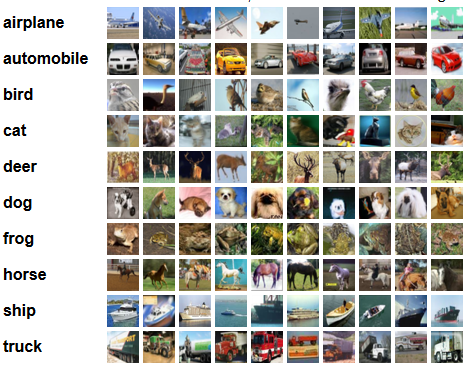
\includegraphics[width=0.8\linewidth]{cifar10}
	\caption{Example of CIFAR-10 images taken from CIFAR website}
\end{figure}

This figure shows some examples of the images that are available in the CIFAR-10 dataset in their respective classes. You will note that 'Truck' and 'Automobile' are both classes of image. However the dataset has been designed such that there is no intersection between classes so a 'Truck' cannot be an automobile and vice-versa.

\subsection{CIFAR-100}
The CIFAR-100 dataset is very similar to CIFAR-10. It contains the same number of images except we now have 100 classes of 600 training images and 20 superclasses for those 100 classes. Each class also includes 100 test images.

Both CIFAR-10 and 100 are created by the same group of people and are based on the same mined internet data.

Due to the lack of training examples and the significantly larger set of classes available, it is a much harder dataset to perform well in with top models getting 75.73 percent accuracy versus 96.53 percent for top performing CIFAR-10 results.

\subsection{The Verdict}
We ended up opting to focus our efforts on CIFAR-10. The reasoning was quite brief. MNIST is too simple and we tackled it early on for test runs. Results were reasonably high.

What we wished to present for our ending point in our project was a classifier which we wanted to use to classify internet images so MNIST wouldn't do for that.

CIFAR-100 on the other hand had features we were interested in trying to work with like the hierarchy which was interesting on the next project we want to do with this model but is quite difficult to get good results with and would push this projects beyond the scope of what can be done in MMP.

CIFAR-10 was a good compromise between the two so it was a good initial goal allowing us to scale to CIFAR-100 if we were satisfied with our results.

\section{Choice of Framework}
To start we need to decide how we are going to implement the neural networks. This involved several steps, of course one would be tempted to write their own implementation for an ANN, however that might be a major project on its own so a better solution is required.

We would like to minimise implementation effort in parts that do not improve the final project as much as possible so a library of some sort is necessary.

For our framework we wanted something that is both performant but also easy to use. We also want support for the latest ANN features while it needs to work on our workstation.

One of the greatest developments of the past 8 years in ANNs and machine learning in general is the advent and wide availability of parallel computing. Specifically GPU compute solutions like nVidia's CUDA technology have been invaluable in making Deep Neural Network research viable offering orders of magnitude better training times. Our frameword must run on a GPU.

We would like a library that makes testing an idea quickly, two modern candidates emerged at that point Google's new Tensor Flow software was one of them and was our favourite for the early parts of the project. Keras was another. Both use Python to define models and a backend implementation to do processing

We were not looking for specific features in this part of our project, what we were looking for however was a framework that is used in current research and is geared towards experimental CNNs both Keras and Tensor Flow support similar advanced CNN features which makes them fairly equivalent as a choice. They were both alpha software when the project started but so are most libraries in the field as CNNs are fairly new. We initially settled on Tensor Flow.

Most of the frameworks for this task are designed to work on Linux primarily. Tensor Flow works on Linux and OSX. This was a problem when we were running Windows on our main machine so the initial solution was to run Tensor Flow on a Virtual Machine with Linux Mint. This initially appeared to work well but we quickly discovered issues with this approach. To get good training performance CUDA is required. However CUDA requires a direct connection to the graphics adapter.

A solution we considered was to use Intel's VT-d and pass the PCI-E device of the GPU directly to the VM using the integrated Intel GPU in Windows instead allowing us to use it under a VM but this proved to be too complicated to set up and any other solution was equally complex. We had to abandon Tensor Flow. Keras, supported Windows as well so we ended up switching our efforts to that. This was relatively early on in the project's lifecycle so we could afford to make the change.

\section{The Stack}
In our architecture we ended up having several layers of software contributing to our final software stack.

\subsection{GPU Drivers and CUDA}
Because of the task of training and running through a neural network is an inherently parallel task we use Nvidia's CUDA technology in order to run computations on the GPU which produces at least an order of magnitude in performance gains over a modern traditional CPU architecture.

Nvidia's CUDA API has emerged as the dominant solution for scientific and industrial compute applications after competing open APIs like OpenCL failed to gain any traction. If you want good ANN performance CUDA is necessary.

\subsection{CuDNN}
CuDNN is an nVidia library written in C++ which provides performance optimisations for several ANN computations to run on CUDA enabled GPUs. This library isn't necessary, but it provided us with a significant performance boost so ended up being invaluable in our experiments.

\subsection{Backend Theano}
To execute computations we are using a library called Theano. Keras interacts with Theano and does weight computations on either the CPU or GPU giving a layer of compatibility and portability to our software as well as provides performance which is essential for training larger models. It uses CuDNN if it's installed to further increase performance on some nVidia GPUs.

\subsection{Keras}
Keras is a framework for creating and testing ANNs. This is the level our code directly interacts with. It provides us with implementations of ANN layers we use to build our models as well as data loaders analytics tools and more.

It can use either Theano or Tensor Flow as a backend to run its computations on the GPU or CPU. Theano then compiles the model in C++ which the CUDA SDK is compatible with.

\subsection{Our Application}
Inside our application we define models and hyper parameters which we are using to test. Our application trains a model and stops when a local minimum is identified for a set span of epochs and then saves the best model ie the local minimum. The model is then evaluated and a classification report is output.

There is methods also for loading models and to use a loaded model to classify an image input. These interfaces can be used to allow an external application to use our system.

\section {The Components of our Application}
Our code is organised in two major structures:
\subsection{Utilities}
This file contains implementations of some image processing algorithms as well as other utility functionality our program needs these are 'features' we use which aren't part of the experiment logic but enable certain experiments to be conducted.
\subsubsection{Colour Conversion}
A useful utility is the ability to convert training example between RGB colour and grayscale. We achieve this by implementing a number of conversion methods to try and extract the luminance of an RGB image. These methods range from averaging the intensity of the RGB channels at their simplest and least effective to weighted averages using the NTSC/W3C and Rec.702 colour weights for each RGB channel.

\subsubsection{Scaling and Cropping}
For this we use a library called OpenCV. Because our neural networks expect inputs to have certain dimensions we must first ensure that the pictures match. Aspect ration must first be matched by cropping trying to get the most prominent object in the cropped frame, then we scale to the desired size using OpenCV's scaling routines to match our ANN inputs.

\subsection{Main Program}
This comes in two separate forms, one is using a simple Multi-Layer Perceptron model and was used early in the project to obtain baseline results, the other is based on a Convolutional Neural Network model and was used in later development. The former was ported over to the framework used in the later for the final results. 

For all intents and purposes information applies to both unless otherwise noted.

\subsection{Challenges and Solutions}

\subsection{Data loading and pre-processing}
The first component of our training framework is loading of data. To do this we are taking advantage of built in Keras data loaders. For CIFAR-10/100 and MNIST these come packaged in and take care of downloading the data as well as loading it if it's not already provided. Tensor Flow and other frameworks also provide this.

After data is loaded we process it such that we extract information from it to determine the shape of the inputs and convert RGB values to a float32 value divided by 255. This gives us our ANN inputs. This is also where we do any splitting and colour conversion.

\subsubsection{Greyscale Luminance}
One of the main advantages and disadvantages of this process is it allows us to reduce the number of inputs into our ANN by a factor of 3. This in turn reduces training time by at least 50 percent which is a good advantage and greatly simplifies our network's structure. At the same time we reduce image detail which can have a negative impact in classification performance.

Because of the tradeoff we use both in our experiments, the faster training and simple models is appealing when trying a new hyper parameter for the first time and want to see quick results. Whereas higher performance is for when we have optimised all other aspects of the network.

We implemented our own colour conversion mechanisms that apply to a single image or sets of images. They are based on documentation for the NTSC and Rec.702 colourspaces as published in their respective standards. Exact references and discussion of the different sources for these are included in appendix 3.

\subsection{The War on Overfitting: State of the Art techniques and Keras}
As we explained in the previous chapter overfitting is a problem for ML and ANNs in particular, in a situation where we wish to achieve the best generalised performance. Training algorithms can only extract patterns from the data which they are given, so it follows that the more we train on data overfitting eventually takes place, i.e our classifier becomes more tailored to the training data at the expense of general performance.

Keras implements many ways to do this but what we are interested in is which ones we should use, in what variation where and how. How do they impact our performance metrics?

\subsubsection{Cross-Validation Split}
One of the most important problems to solve when combating overfitting is to be able to determine when it is happening so we may act on it.

What Keras enables us to do is to provide a set for validation which we can test against after each training epoch while we monitor our loss to train on our training data. Keras also has a feature to split a portion of the nth portion of the data for this purpose.

Our implementation is to use Keras's validation split for normal data and our own implementation for augmented data. This is because Keras until recently did not provide this feature for its data generator. In CIFAR-10 and 100 data is randomly distributed so we can just split the data at a point from the end and use that for this purpose.

What we do instead is we first shuffle in parallel the training data and labels then split the nth portion at the end. This approach would have been more useful if we were averaging runs. As it stands it means we have unnecessary variations in our data but our results were not visibly affected by this, we could have re-designed this omitting the shuffling or storing the seed for repeatability, but ideally we'd use Kera's better implementation instead now that it's available.

\subsubsection{Early Stopping and  Model Checkpoint}
Once we can monitor validation loss and can detect when a model might be overfitting we need something to act upon this. These methods are what we use.

Keras has a callback interface that allows us to call code in certain instances during training to do things. Early Stopping allows us to, with a patience parameter stop training when a model's validation results stop improving for a certain number of epochs. We use 50 epochs in most of our experiments. Because of how training works we want patience to be higher to avoid local minima since what we are looking for is actual local minimum validation loss.

Model checkpoint on the other hand solves another related issue. When validation results stop improving we stop after a few epochs but actually our best result might be several epochs old by the time we stop which means our model will already show signs of overfitting by the time it stops. We can avoid this issue by saving a copy of our most general model and loading it after our training has stopped and use that for validation.

\subsubsection{Data Augmentation}
Keras provides a capability to pass training data through a data generator before they are fed to the neural network for training. The idea is you can set filters that get applied randomly on each image such that every time you encounter an image in training it is slightly different in appearance.

The way this works is that by changing the actual pixel data in the inputs just enough so that the image features are intact you can mitigate the neural network overfitting to the data somewhat.

What we use is random rotation, which rotates the the image around its centrer by a random value of a given range, e.g. -1-1 degrees. Horizontal flip, which flips the image horizontally with a 50 percent likelyhood, and shifting the image by 2 pixels in either direction thus re-positioning it.

The filters work cyclically such that for n images n+1 image will be image 1 but each time the parameters of the filters will vary.

Another later consideration which came from a thought when we were examining data augmentation was to apply random noise to the inputs in hopes of reducing overfitting using the same principle. Keras does support the feature as a normalisation layer but at that point we already had data augmentation implemented and we found out that this kind of augmentation would be ill suited to the very small images we have in our network.

\subsubsection{Dropout}
We are using Keras implementation of dropout to reduce overfitting.

\subsection{Obtaining and visualising results}
For our experiments to be worth their salt we need to be able evaluate our models and visualise our results. For this we turn to SciKit Learn, which is an excellent library for machine learning statistics and visualisations. It helps us generate classification reports and confusion matrices which is the basis of our result reporting.

We also initially intended to have a Google Inception-like visualisation of the learned features but we run out of time before implementing this.
\chapter{Results and Conclusions}
In this section we will describe our results and any conclusions we may have drawn from them as well as decisions that came from these results.
\section{Convolutional Neural Networks: Results}
All the neural network here are conv nx3x3 - conv nx3x3 - max pool 2x2 no strides - conv nx3x3 - conv nx3x3 - max pool 2x2 no strides - Dense 256 - Dense 128 - Dense Softmax 10 with Relu activations in the rest of the layers. Where this is not true we will note as such
\subsection{Number of Filters}
For this we are evaluating the following models:
\begin{itemize}
	\item 8-8-14-14 with 3x3 filters
	\item 24-24-32-32 with 3x3 filters
	\item 32-32-64-64 with 3x3 filters
	\item 48-48-96-96 with 3x3 filters
	\item 128-128-256-256 with 3x3 filters
\end{itemize}
For the results we are presenting here we are using data augmentation in all cases to reduce overfitting as well as early stopping to get the best model possible from our training. We have results for both colour and black and white for this evaluation.

We will only be presenting the colour results in this part as we will be evaluating the impact of colour in a later part.

\subsubsection{Effects on Training Speed}
As we increase the amount of filters we see our training speed declining as the number of neurons increases, this makes sense as you increase the number of computations that need to be done each epoch somewhat.

We ommit actual data here we were unable to control running parameters exactly due to these tests having to be run over several nights at different system workloads which would affect the results but our observations showed that we can get a range of 12s per epoch on our smallest model to 57s per epoch on our most complicated model
\subsubsection{Effects on Performance}
We begin this investigation assuming we will get better results with more. 
\begin{figure}
	\begin{tabular}{cc}
		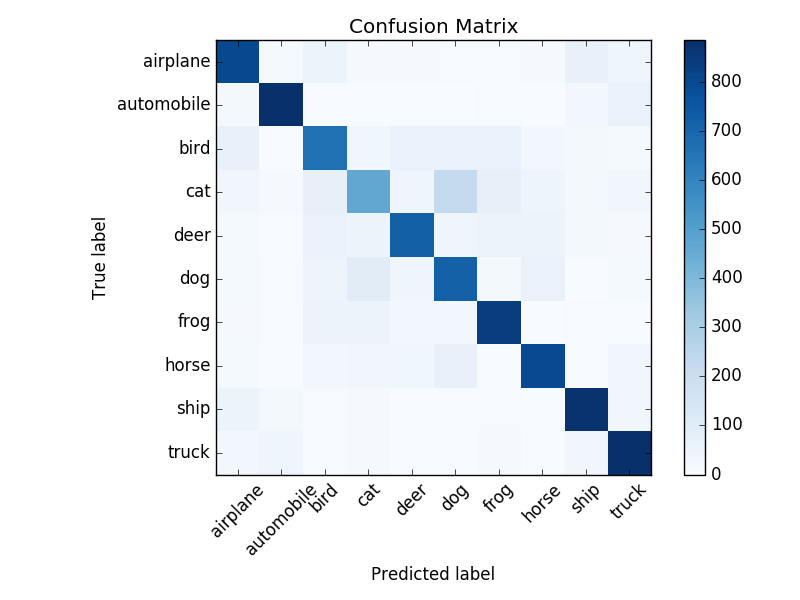
\includegraphics[width=0.45\linewidth]{8-8-14-14-3x3-15pct-color_confusion_matrix} &   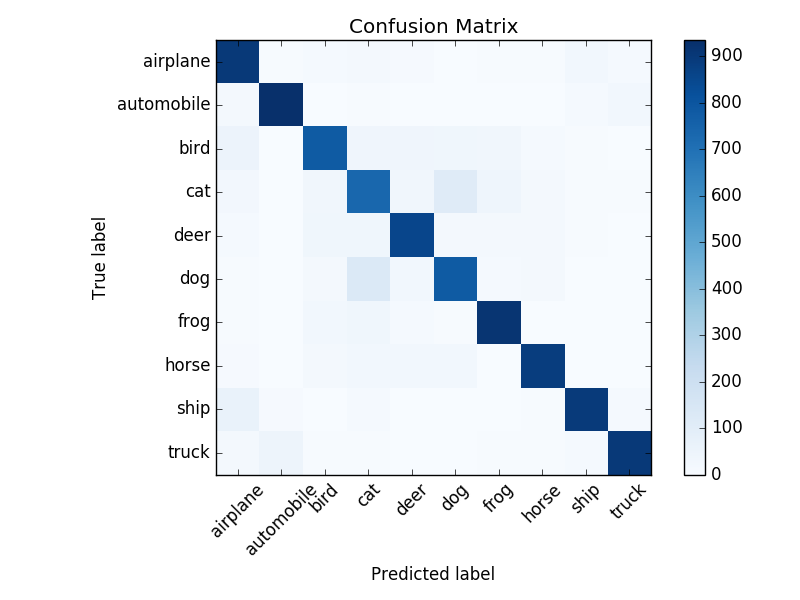
\includegraphics[width=0.45\linewidth]{24-24-48-48-3x3-15pct-color_confusion_matrix} \\
		(a) 8-8-14-14 & (b) 24-24-32-32 \\[6pt]
		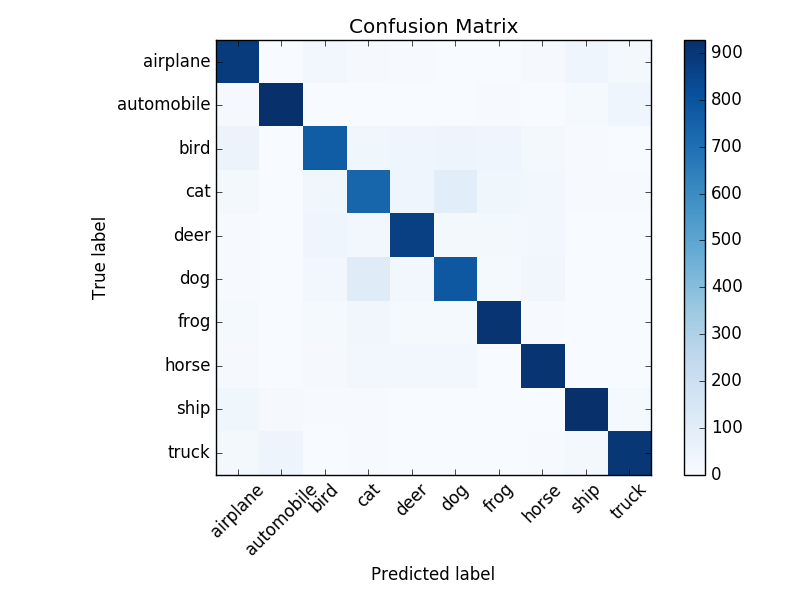
\includegraphics[width=0.45\linewidth]{32-32-64-64-3x3-15pct-color_confusion_matrix} &   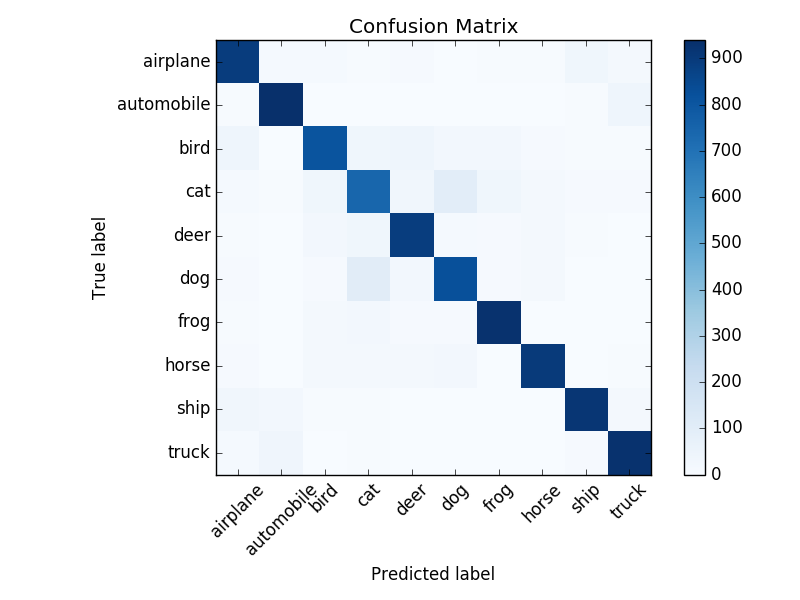
\includegraphics[width=0.45\linewidth]{48-48-96-96-3x3-15pct-color_confusion_matrix} \\
		(c) 32-32-64-64 & (d) 48-48-96-96 \\[6pt]
		\multicolumn{2}{c}{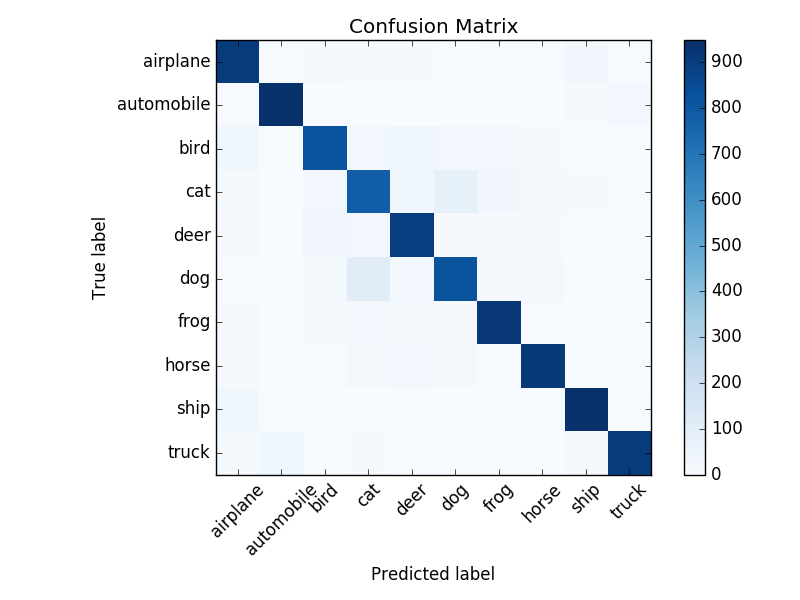
\includegraphics[width=0.45\linewidth]{128-128-256-256-3x3-15pct-no-strides-color_confusion_matrix} }\\
		\multicolumn{2}{c}{(e) 128-128-256-256}
	\end{tabular}
	\caption{Confusion Matrices varied by filter number}
\end{figure}

As we can see from the figures, a significant improvement between out smallest model and out largest one. However it appears we hit diminishing returns after a certain number of filters as we presumably hit the limit of the features we can draw from our small 32x32 data.

From the qualification report we also see an interesting pattern we hinted on earlier in this document. Dogs and Cats are the worst performing classes with confusing happening mostly between them but dogs get confused less with cats than the opposite.

This becomes clearer when we look at the classification reports.
\begin{figure}
\begin{verbatim}
8-8-14-14:
             precision    recall  f1-score   support
             
          0       0.78      0.72      0.75      1000
          1       0.84      0.90      0.87      1000
          2       0.67      0.55      0.61      1000
          3       0.55      0.45      0.50      1000
          4       0.64      0.72      0.68      1000
          5       0.63      0.65      0.64      1000
          6       0.73      0.83      0.77      1000
          7       0.74      0.81      0.77      1000
          8       0.80      0.84      0.82      1000
          9       0.86      0.82      0.84      1000
             
   avg / total       0.73      0.73      0.73     10000
\end{verbatim}
\begin{verbatim}  
24-24-48-48:
             precision    recall  f1-score   support
             
          0       0.82      0.90      0.86      1000
          1       0.93      0.94      0.93      1000
          2       0.84      0.78      0.81      1000
          3       0.71      0.74      0.72      1000
          4       0.85      0.86      0.86      1000
          5       0.79      0.78      0.79      1000
          6       0.88      0.91      0.90      1000
          7       0.91      0.89      0.90      1000
          8       0.93      0.90      0.91      1000
          9       0.94      0.90      0.92      1000
             
   avg / total       0.86      0.86      0.86     10000
\end{verbatim}
\begin{verbatim}    
32-32-64-64:
             precision    recall  f1-score   support
             
          0       0.84      0.89      0.86      1000
          1       0.94      0.93      0.93      1000
          2       0.83      0.77      0.80      1000
          3       0.74      0.74      0.74      1000
          4       0.85      0.87      0.86      1000
          5       0.80      0.79      0.79      1000
          6       0.89      0.91      0.90      1000
          7       0.89      0.91      0.90      1000
          8       0.91      0.93      0.92      1000
          9       0.92      0.90      0.91      1000
             
   avg / total       0.86      0.86      0.86     10000
\end{verbatim}
\begin{verbatim}  
48-48-96-96:  
             precision    recall  f1-score   support
             
          0       0.87      0.89      0.88      1000
          1       0.92      0.94      0.93      1000
          2       0.87      0.81      0.84      1000
          3       0.76      0.74      0.75      1000
          4       0.86      0.89      0.88      1000
          5       0.83      0.82      0.83      1000
          6       0.91      0.93      0.92      1000
          7       0.92      0.90      0.91      1000
          8       0.92      0.92      0.92      1000
          9       0.90      0.93      0.92      1000
             
    avg / total       0.88      0.88      0.88     10000
\end{verbatim}
\begin{verbatim}  
128-128-256-256:
             precision    recall  f1-score   support
             
          0       0.87      0.91      0.89      1000
          1       0.95      0.95      0.95      1000
          2       0.87      0.82      0.84      1000
          3       0.77      0.78      0.78      1000
          4       0.85      0.89      0.87      1000
          5       0.85      0.82      0.83      1000
          6       0.90      0.92      0.91      1000
          7       0.93      0.92      0.92      1000
          8       0.92      0.94      0.93      1000
          9       0.96      0.91      0.93      1000
             
   avg / total       0.89      0.89      0.88     10000
\end{verbatim}
\caption{Classification Reports for experiments}
\end{figure}

As you might notice from the figures above we stop seeing overall improvements at 48-48-96-96 with small improvement in some classes, but the extra cost of the larger networks makes it a good compromise for further experiments.
\subsubsection{Effects on Size of Weights}
This investigation is much simpler. We look at the sizes of the weights we store for each network and try to correlate it the number of calculations and network complexity.
\begin{figure}
	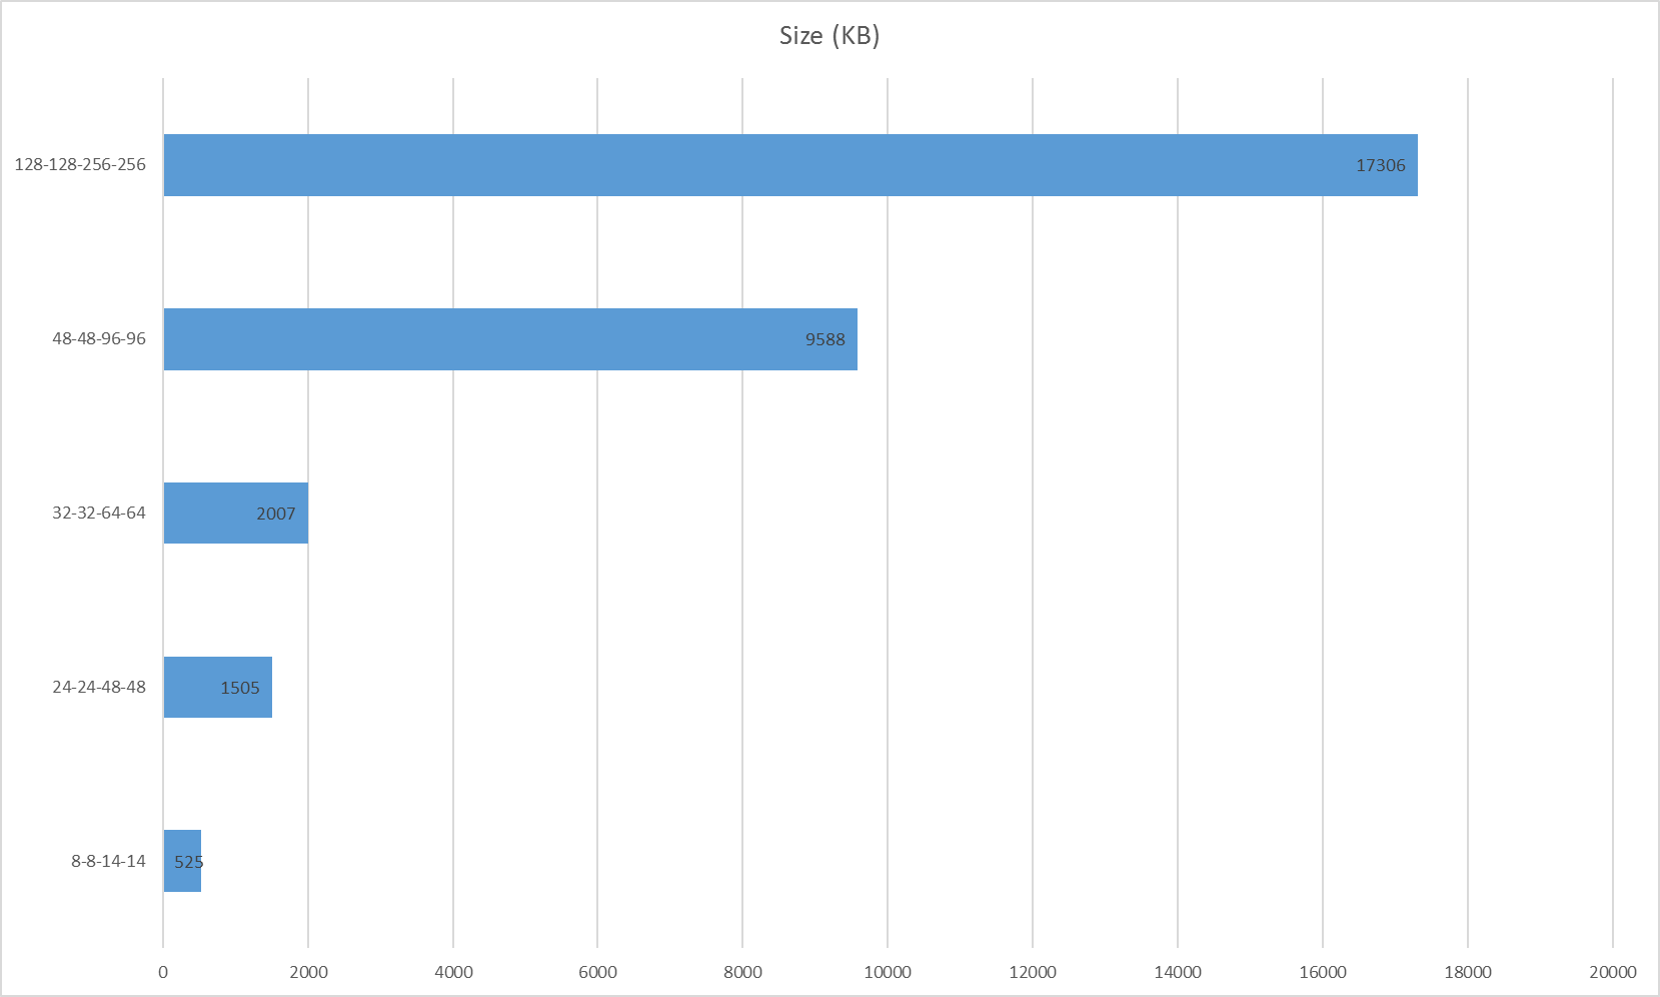
\includegraphics[width=0.8\linewidth]{datasizes_filters}
	\caption{Bar Chart of Size of Stored Weights}
\end{figure}

\subsection{Size of Filters}
\subsubsection{Effects on Training Speed}
\subsubsection{Effects on Performance}
\subsubsection{Effects on Size of Weights}

\subsection{Number of Colour Channels}
\subsubsection{Effects on Training Speed}
\subsubsection{Effects on Performance}
\subsubsection{Effects on Size of Weights}

\subsection{Number of Hidden Layers}
\subsubsection{Effects on Training Speed}
\subsubsection{Effects on Performance}
\subsubsection{Effects on Size of Weights}

\subsection{Augmentation}
\subsubsection{Effects on Training Speed}
\subsubsection{Effects on Overfitting}
\subsubsection{Effects on Performance}

\subsection{Multi Layer Perceptron: Figures in Matrices}

\section{Miscellaneous Discussion}
\subsection{Accounts of Early Experiments}
Here we will discuss the earliest parts of our experimentation. These were done before the experimental infastructure was complete so we don't have complete figures recorded for them. These accounts are based on logs and diary entries taken at the time. Rapid prototyping was taking place at the time so results might not be consistent. As a result this section is included in a pure discussion format and is aimed to offer some insight to early decisions taken in this project.

\subsubsection{Early Experiments}
% add any additional chapters here

\setemptyheader
\addcontentsline{toc}{chapter}{Appendices}
\chapter*{Appendices}
\pagebreak

% start the appendix - sets up different numbering
\fancypagestyle{plain}{%
%\fancyhf{} % clear all header and footer fields
\fancyhead[L]{\textsl{Appendix\ \thechapter}}
\fancyhead[R]{\textsl{\leftmark}}}

\appendix
\fancyhead[L]{\textsl{Appendix\ \thechapter}}
\fancyhead[R]{\textsl{\leftmark}}
\fancyhead[C]{}
\fancyfoot[C]{\thepage}
\renewcommand{\headrulewidth}{0.4pt}
\renewcommand{\chaptermark}[1]{\markboth{#1}{}}

\fancyhead[L]{\textsl{Appendix\ \thechapter}}
\fancyhead[R]{\textsl{\leftmark}}
\fancyfoot[C]{{\thepage} of \pageref{LastPage}}

% include any appendices here
\chapter{Third-Party Code and Libraries}

If you have made use of any third party code or software libraries, i.e. any code that you have not designed and written yourself, then you must include this appendix. 

As has been said in lectures, it is acceptable and likely that you will make use of third-party code and software libraries. The key requirement is that we understand what is your original work and what work is based on that of other people. 

Therefore, you need to clearly state what you have used and where the original material can be found. Also, if you have made any changes to the original versions, you must explain what you have changed. 

As an example, you might include a definition such as: 

Apache POI library � The project has been used to read and write Microsoft Excel files (XLS) as part of the interaction with the client�s existing system for processing data. Version 3.10-FINAL was used. The library is open source and it is available from the Apache Software Foundation 
\cite{apache_poi}. The library is released using the Apache License 
\cite{apache_license}. This library was used without modification. 

\chapter{Ethics Submission}
\section{Submission Number 4111}


\includepdf[pages={-}]{./Appendix2/4111.pdf}
\chapter{Code Examples}

\section{Colour Conversion}

This code enables conversion between RGB channel intensities into greyscale luminance using different conversion methods based on their respective colourspace recommendations in a variety of modes. A starting discussion on the effects of different methods can be found \hyperlink{http://cadik.posvete.cz/color_to_gray_evaluation/}{here}

\begin{lstlisting}
import numpy as np
from math import sqrt

def convert_set_to_greyscale(cifar_set, method=0, gamma=1.0):
	converted_set = np.empty((cifar_set.shape[0], 1, cifar_set.shape[2], cifar_set.shape[3]), 'float32')
	for image_index, image in enumerate(cifar_set):
		for row_index, row in enumerate(image[0]):
			for pixel_index, pixel in enumerate(row):
			grey = 0.0
			if method == 0:  # Rec.709 luminance
				grey = (0.2126 * cifar_set[image_index, 0, row_index, pixel_index]) + \
				(0.7152 * cifar_set[image_index, 1, row_index, pixel_index]) + \
				(0.0722 * cifar_set[image_index, 2, row_index, pixel_index])
			elif method == 1:  # NTSC/W3C luminance
				grey = (0.299 * cifar_set[image_index, 0, row_index, pixel_index]) + \
				(0.587 * cifar_set[image_index, 1, row_index, pixel_index]) + \
				(0.114 * cifar_set[image_index, 2, row_index, pixel_index])
			elif method == 2:
				grey = sqrt(((0.299 * cifar_set[image_index, 0, row_index, pixel_index]) ** 2) +
				((0.587 * cifar_set[image_index, 1, row_index, pixel_index]) ** 2) +
				((0.114 * cifar_set[image_index, 2, row_index, pixel_index]) ** 2))
			elif method == 3:
				grey = sqrt(((0.2126 * cifar_set[image_index, 0, row_index, pixel_index]) ** 2) +
				((0.7152 * cifar_set[image_index, 1, row_index, pixel_index]) ** 2) +
				((0.0722 * cifar_set[image_index, 2, row_index, pixel_index]) ** 2))
			elif method == 4:  # Simple mean of RGB
				grey = ((cifar_set[image_index, 0, row_index, pixel_index]) +
				(cifar_set[image_index, 1, row_index, pixel_index]) +
				(cifar_set[image_index, 2, row_index, pixel_index])) / 3
			else:
				print 'Error: This is not a valid conversion mode.\n Reverting to colour.'
			return cifar_set.astype('float32') / 255
		
		converted_set[image_index, 0, row_index, pixel_index] = np.float32(grey/255)
	print 'Converted ', len(converted_set), ' images to greyscale.'
	return converted_set
 
\end{lstlisting}


\fancypagestyle{plain}{%
   \fancyhead{} %[C]{Annotated Bibliography}
   \fancyfoot[C]{{\thepage} of \pageref{LastPage}} % except the center
   \renewcommand{\headrulewidth}{0pt}
   \renewcommand{\footrulewidth}{0pt}
}

\setemptyheader

\nocite{*} % include everything from the bibliography, irrespective of whether it has been referenced.

% the following line is included so that the bibliography is also shown in the table of contents. There is the possibility that this is added to the previous page for the bibliography. To address this, a newline is added so that it appears on the first page for the bibliography. 
\addcontentsline{toc}{chapter}{Annotated Bibliography} % Adds References to contents page

%
% example of including an annotated bibliography. The current style is an author date one. If you want to change, comment out the line and uncomment the subsequent line. You should also modify the packages included at the top (see the notes earlier in the file) and then trash your aux files and re-run. 
%\bibliographystyle{authordate2annot}
\bibliographystyle{IEEEannot}
\renewcommand{\bibname}{Annotated Bibliography} 
\bibliography{References/references} % References file


\end{document}
